\subsection{Driver circuitry and optocouplers}  \label{driver}

The control signal is generated by the control platform, which consists on a Plexim RTbox. In order to provide galvanic isolation between the converter and the control signal generator, optocouplers are used. The chosen optocoupler is the ACPL-W70L-000E\todo{include datasheet AT}. This optocoupler includes output signal circuitry which allows saving a pull-up or pull-down resistor. The IC is not an open collector device. Its main features might be seen at \ref{opto_features}.

\begin{table}[htbp]
	\centering
	\begin{tabular}{|p{6cm}|>{\centering}p{8cm}|}
		\hline
		\rowcolor{lightgray}\multicolumn{2}{|l|}{ \textbf{Maximum ratings}} \\ \hline
		Supply voltage & 6 [V]  \tabularnewline \hline
		Average input current & 10 [mA]  \tabularnewline \hline
		Average output current & 10 [mA]  \tabularnewline \hline
		\rowcolor{lightgray}\multicolumn{2}{|l|}{ \textbf{Other values of interest}} \\ \hline
		Input forward voltage & 1.5 [V]  \tabularnewline \hline
		Package & SSOIC6  \tabularnewline \hline
	\end{tabular}
	\caption{Optocoupler figures of merit.
	\cite{opto_datasheet}}
	\label{opto_features}
\end{table}
\todo{If it is maxiumum ratings why is it also average output and average input? AT}

The signal from the optocoupler has to be amplified in order to drive the switches. The driver provides voltage amplification and current capability. The chosen IC to perform the task is NCP81074\todo{include datasheet AT}. Find in table \ref{driver_features} its main features. 

\begin{table}[htbp]
	\centering
	\begin{tabular}{|p{6cm}|>{\centering}p{8cm}|}
		\hline
		\rowcolor{lightgray}\multicolumn{2}{|l|}{ \textbf{Maximum ratings}} \\ \hline
		Supply voltage & 24 [V]  \tabularnewline \hline
		Output current (pulse < 0.5 $\mu$s) & 10 [A]  \tabularnewline \hline		
		Reverse current (pulse < 1 $\mu$s) & 10 [A]  \tabularnewline \hline
		Input signal voltage & -6 to 24 [V]  \tabularnewline \hline
		\rowcolor{lightgray}\multicolumn{2}{|l|}{ \textbf{Other values of interest}} \\ \hline
		Output resistance & 0.4 [$\Omega$]  \tabularnewline \hline
		Package & SOIC8  \tabularnewline \hline
	\end{tabular}
	\caption{Driver figures of merit.
		\cite{driver_datasheet}}
	\label{driver_features}
\end{table}

As the MOSFET is a voltage controlled switch, the voltage between the gate and the source, $V_{GS}$ must be equal to its characteristic $V_{th}$ in order to allow current flow. The dynamics of the switching can be modelled as a simple RC circuit, see figure \ref{mosfet_rc_gate}.


\begin{figure}[htbp]
	\begin{center}
		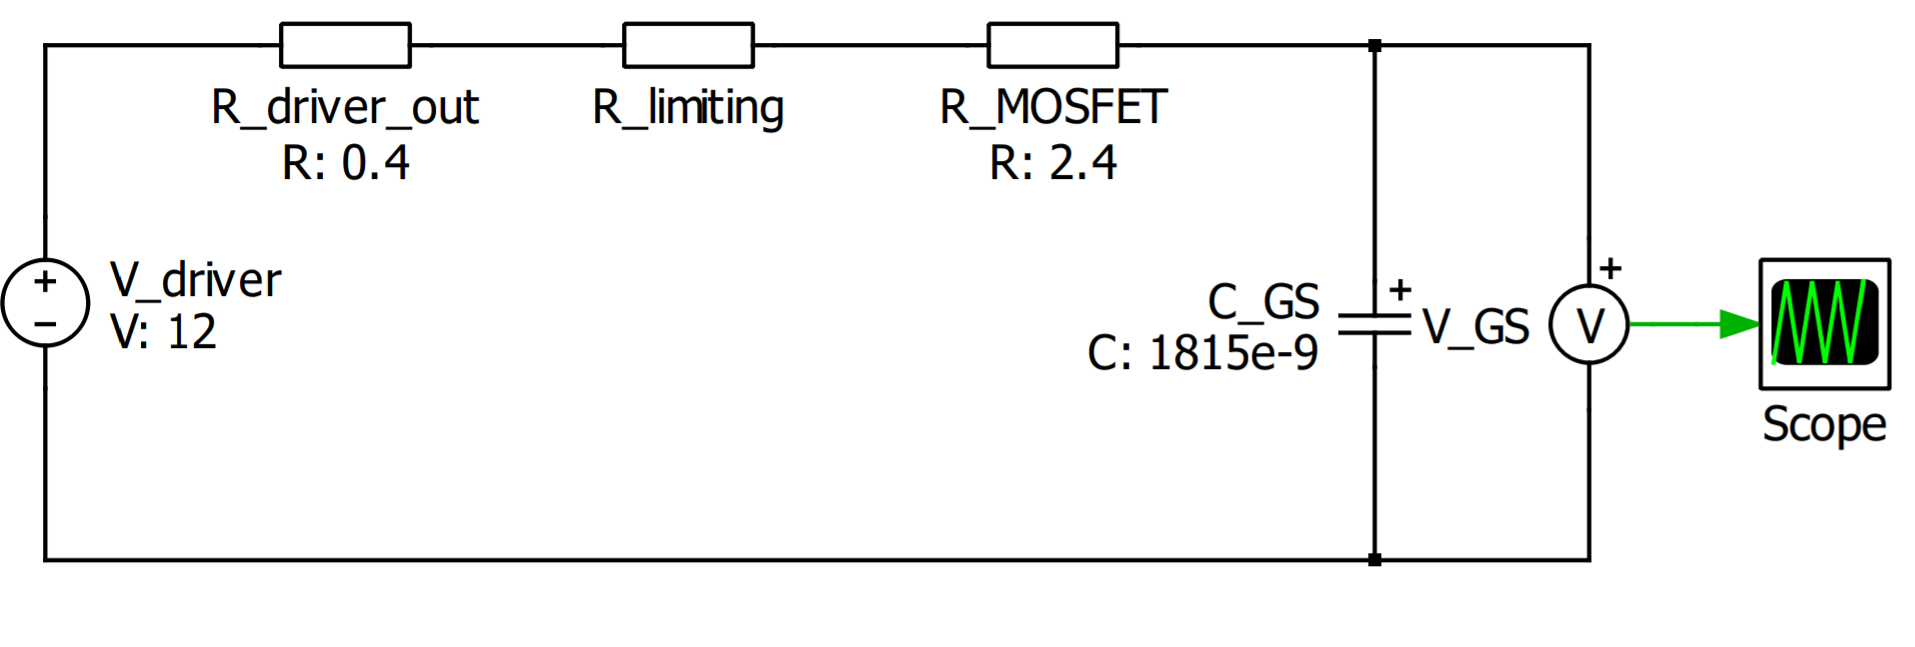
\includegraphics[width=0.4\textwidth]{../Pictures/P1/driver_resistor_sizing.png}
		\caption{Simplified circuit used to model the MOSFET switching dynamics.}
		\label{mosfet_rc_gate}
	\end{center}	
\end{figure}
\todo{This figure is way to small, but also revise others. AT}



*why driver circuitry
*different driver grounds --> solution, no bootstrap
*gate pull down resistor
*gate resistor sizing, effect over switching frequency 
*calculated/simulated switching losses
*layout considerations
*pull down resistors

